%=========================================================================

\chapter{Introduction}
This chapter describes the motivation leading to the presentation of this thesis and how is it related to the SLAM++ project at FIT VUT. The objectives of the project and the subjects included in this document are briefly explained. The chapter ends describing the overall structure and contents of the remaining of the thesis.

\section{Motivation}
There is an immerse need to record and preserve our knowledge and perception of the world around us. Evidence of such tendency can be track thousands of years back in human existence as a cave paintings. Later we used more advanced techniques in form of written languages, sculptures, drawings etc. Nowadays we have means to record our surroundings as we perceive it in 2D using cameras. However, it has proven difficult to process such information digitally. Even automated analysis of 2D information like typeset books is not a trivial problem and far from being mastered. While there are so called OCR converters available, in many cases they don't work reliably enough.

When it comes to 3D the problem gets much more difficult. Scanning 3D object reliably is nowadays possible in laboratory conditions, but there are hard limits like the size of the object, its structure or surface and material properties. Also the laboratory equipment used is much more expensive and physically larger compared to its 2D counterpart. This thesis tries to address both of these problems by allowing user to create 3D model using pictures of an object of interest from various sources. Such 3D model, even though it may be inaccurate, has number of applications. It can be used by archaeologists to preserve cultural heritage, by architects for spatial planning, by entertainers to create 3D models and virtual reality or by engineers to replicate existing 3D objects.

\section{Tools}
The process of creating a 3D model usually consist of two parts: scanning the object and reconstruction of the model. There are three main approaches how to scan physical object: contact, active non-contact  and passive non-contact scanners. The contact 3D scanners probe the subject through physical touch. The active non-contact scanners use a light in forms of laser or X-ray to scan the object while the passive non-contact scanners are using either multiple cameras, images with varying lighting conditions or silhouettes extruded from image with contrasted background. In this thesis we will be particularly interested in scanning objects using multiple images from various cameras. We will talk more about this in next chapter \ref{chapter:theoretical-background} but for now note that for this we will use the SLAM++ framework \cite{www:slam}. The output of such scanning is usually a set of 3D points with a color information called point cloud. These data have to be filtered in order to remove noise , segmented and then reconstructed into polygonal model. This can be either done manually using software like MeshLab \cite{www:meshlab} or automatized with the PCL framework \cite{www:pcl}. 

\section{Objectives}
The thesis aims to identify challenges of 3D reconstruction from a set of 2D images taken by various cameras and create a software to do so automatically. This objective deals with the study of camera modelling and calibration and the comprehension of epipolar geometry. Then, the computation of the fundamental matrix of a multiple images system is surveyed with the aim of reducing the correspondence problem between each two images. An accurate estimation of the fundamental matrix allows us to compute 3D information about objects depicted and validate it. In order to eliminate artefacts the input set of images, obtained from internet, will have to be filtered to contain only daytime images from summer season.

The study of the geometry involved in multiple camera vision systems should allow us to present an application that can from a set of images reconstruct 3D scene where they were taken in.

\section{Overall Structure}
This thesis consist of X chapters, Y appendices and a bibliography at the end of the document.

Chapter \ref{chapter:theoretical-background} focuses on providing necessary theoretical knowledge required to understand principle of 3D reconstruction from 2D images. It explains the calibration parameters of the camera model and optic characteristics of the image. Second, it introduces epipolar geometry and its role in 3D reconstruction along with fundamental matrix. Then the features extraction and matching techniques are briefly discussed. Once such knowledge is presented, it explains what are the passive non-contact scanning 3D techniques used starting with stereo vision, mono vision and lastly the uncalibrated camera approach.

Chapter \ref{chapter:the-state-of-the-art} discusses existing software and presents results it outputs. It firstly explains and compares various features detectors, extractors and matchers that are built in the SLAM++ frontend. The comparison is then discussed and best combination in terms of performance and effectiveness chosen for the resulting application. Next we discuss existing competitive solutions, namely VisualSFM, photosynth and Bundler. These will be used for the final application performance and effectiveness evaluation.

In the chapter \ref{chapter:methodology} the whole 3D reconstruction process is outlined and step by step explained. It consists of steps. First it discusses features detection and extraction. Then the features are being matched and filtered using the RUNSAC algorithm. The output is used to calculate the fundamental matrix and camera model using mathematical apparatus from chapter \ref{chapter:theoretical-background}. Finally, once the camera model is estimated, dense reconstruction is run creating the resulting point cloud.

Chapter \ref{chapter:results_evaluation} evaluates experimental results from the implemented solution. It elaborates on  the effectiveness to performance ratio of the uncalibrated app with competition.

Finally, chapter \ref{chapter:conclusion} summarizes this document by discussing achieved goals and comparisons to existing solutions.

\chapter{Theoretical Background}
\label{chapter:theoretical-background}
In this chapter reader will be introduced to the mathematical apparatus used in 3D model reconstruction. Firstly we will talk about the camera model and calibration and why is it crucial component for further scene reconstruction. Then the epipolar geometry along with fundamental matrix estimation are discussed as these describe the relationship between each set of two viewspoints. Next we will introduce the detection of features in images, their extraction and matching such points between two images. Lastly the passive non-contact scanning techniques are discussed using stereo vision, one calibrated moving camera and a set of uncalibrated cameras.
\section{Mathematical Model}
\subsection*{Camera Model and Calibration}
\subsection*{Epipolar Geometry}
\subsection*{Fundamental Matrix}
\section{Feature Based Image Registration}
\section{3D Reconstruction Approaches}
Stereo, Mono, Uncalibrated

\chapter{The State of the Art}
\label{chapter:the-state-of-the-art}
The following chapter evaluates various detectors, extractors and matchers in order to choose the best combination in terms of performance and effectiveness for reconstruction of historic landmarks. Then the already existing 3D reconstruction software is introduced and briefly evaluated. Some of the programs will be later used to evaluate effectiveness and performance of our program.

\section{Detectors}
A successful 3D reconstruction stands and falls on good features detection.The quality and robustness of features is (usually) much more important then their quantity which will be demonstrated by the Dense detector later in this section. The ideal feature detector finds salient image regions such that they are repeatedly detected despite change of viewpoint; more generally it is robust to all possible image transformations. Therefore, it does not detect any points in uniform and uninteresting surfaces like sky or texture-less walls. The best detector to be used depends heavily on the requested task. In our application features we are interested in are edges and corners of buildings and their distinct parts.

We can divide types of image features into following categories (please note that a detector can detect features from multiple categories):
% CITATION NEEDED!!!
\begin{itemize}
	\item \textbf{Edge} is a point where there is a sudden change between adjacent pixels (strong gradient magnitude). Generally an edge can be of almost any arbitrary shape and may include junctions. Locally edges have a one-dimensional structure.
	\item \textbf{Interest point} has a local two dimensional structure. We can think of it as two-dimensional edge, in fact early algorithms were used to detect interest points as edges and then selected the interest points by further calculation. In some literature you the interest points may be referred to as corners.
	\item \textbf{Blobs} provide a complementary description of image structures in terms of regions, as opposed to corners that are more point-like. A term regions of interest or interest points are sometimes used as the blob descriptors often contain a preferred point (a local maximum or a center of gravity). Blobs allows detection of smooth areas in an image that might not be detected as an edge or corner.
	\item \textbf{Ridges} are in computer vision a set of curves whose points are, in one or more ways to be made precise below, local maxima of the function in at least one dimension. This notion captures the intuition of geographical ridges. Ridge detection is usually much harder then Edge, Interest point or Blob detection.
\end{itemize}

In the remainder of this section feature detectors implemented in OpenCV will be presented. Each detector will be run with on same set of images with historic landmarks in order to evaluate the effectiveness and speed. Then a summary of the results will be presented.
 
\begin{itemize}
	\item The \textbf{Robust Invariant Scalable Keypoints (BRISK)} detector uses scale-space pyramid layers of octaves and intra-octaves to detect corners in an image. The algorithm uses FAST feature detector score and was developed to get the better of SIFT and SURF detectors. However, in our case the performance gain is not worth decreased feature quality. \cite{article:brisk}
\end{itemize} 

\subsection*{DENSE}
\subsection*{FAST}
\subsection*{GFTT}
\subsection*{HARRIS}
\subsection*{MSER}
\subsection*{ORB}
\subsection*{SIFT}
\subsection*{Simple BLOB}
\subsection*{SURF}

\section{Extractors}
Once features have been detected, a local image patch around the feature can be extracted. This extraction may involve quite considerable amounts of image processing. The result is known as a feature descriptor or feature vector. Among the approaches that are used to feature description, one can mention N-jets and local histograms. In addition to such attribute information, the feature detection step by itself may also provide complementary attributes, such as the edge orientation and gradient magnitude in edge detection and the polarity and the strength of the blob in blob detection.

\begin{itemize}
	\item \textbf{SIFT:} The scale-invariant feature transform of a neighbourhood is a 128-dimensional vector of histograms of image gradients. The region, at the appropriate scale and orientation, is divided into a $4\times 4$ square grid, each cell of which yields a histogram with 8 orientation bins.
\end{itemize}
\section{Matchers}

\section{Existing 3D Reconstruction Solutions}
The problem of creating 3D reconstruction from set of images has been addressed by several other groups. There are some 
\subsection*{Photosynth}
Photosynth is a software application developed by Microsoft. It is based on Photo Tourism, a research project by University of Washington graduate student Noah Snavely. Formerly the Photosynth was a 3D reconstruction software, however, in the current version output of the application is not a point cloud nor 3D model but an animation of morphing images or panorama. While it still works with images from various sources, the best result is achieved by importing photos from a single camera. Once imported, user has to choose the camera trajectory from four predefined options: spin, panorama, wall or walk. 

The Photosynth technology is using an interest point detection and matching algorithm developed by Microsoft Research which is similar in function to SIFT. Detected features are then matched between images and by analyzing subtle differences in the relationships between the features (angle, distance, etc.), the program identifies the 3D position of each feature, as well as the position and angle at which each photograph was taken. Everything is processed by Microsoft's servers and, once finished, pushed to the website or desktop/mobile application. There are little to none information about the whole process as this is a commercialized technology. \cite{www:photosynth}

\begin{figure}[ht]
	\begin{center}
		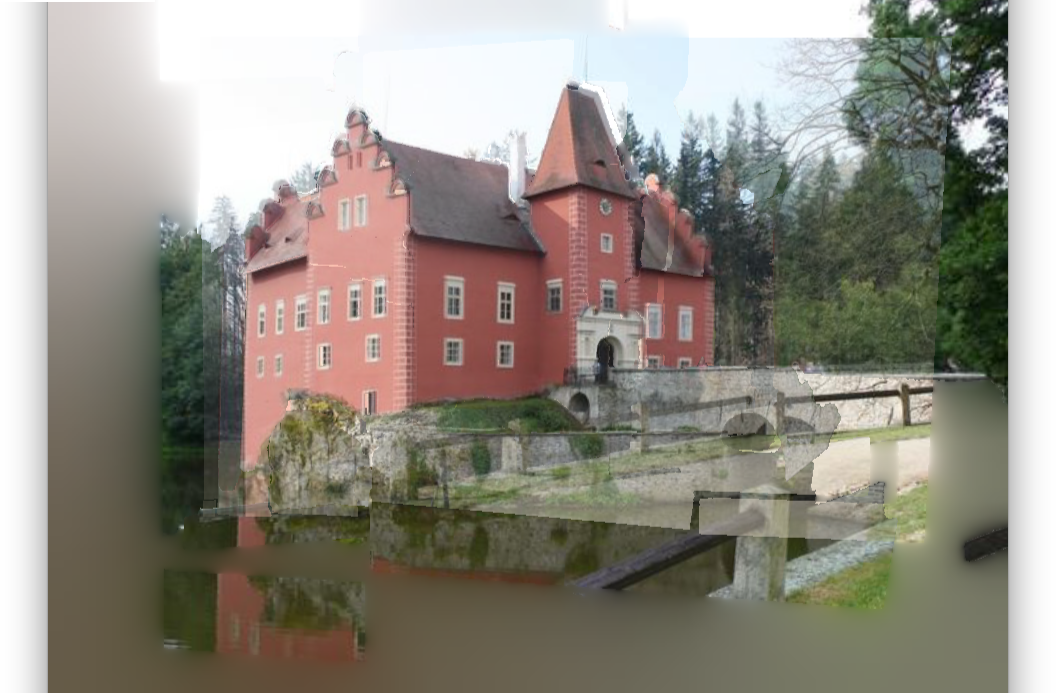
\includegraphics[keepaspectratio,width=14cm]{fig/Photosynth.png}
	\end{center}
	\caption{The Photosynth output of the Červená Lhota Castle in transition between several morphed images.}
	\label{fig:visualsfm}
\end{figure}

\subsection*{VisualSFM}
The Chungchang Wu's Visual Structure from Motion System is a GUI application for 3D reconstruction using structure from motion (SFM). The reconstruction system is modular and integrates several of other projects: SIFT on GPU(SiftGPU), Multicore Bundle Adjustment, and Towards Linear-time Incremental Structure from Motion. VisualSFM runs fast by exploiting multicore parallelism for feature detection, feature matching, and bundle adjustment. For dense reconstruction, the program supports Yasutaka Furukawa's PMVS/CMVS tool chain, and can prepare data for Michal Jancosek's CMP-MVS. In addition, the output of VisualSFM is natively supported by Mathias Rothermel and Konrad Wenzel's SURE.

The software follows the overall 3D reconstruction pipeline; It detects features using SIFT detector and SIFT extractor, matches feature pairs with the N-View Match, estimates the camera model for each image, removes images' distortion and then runs the dense reconstruction. Outputs of feature extraction and matching are stored as a binary files and are loaded if provided to save processing time. This enables use of other than built-in extractors and matcher, at least for the sparse reconstruction. \cite{www:visual_sfm}

\begin{figure}[ht]
	\begin{center}
		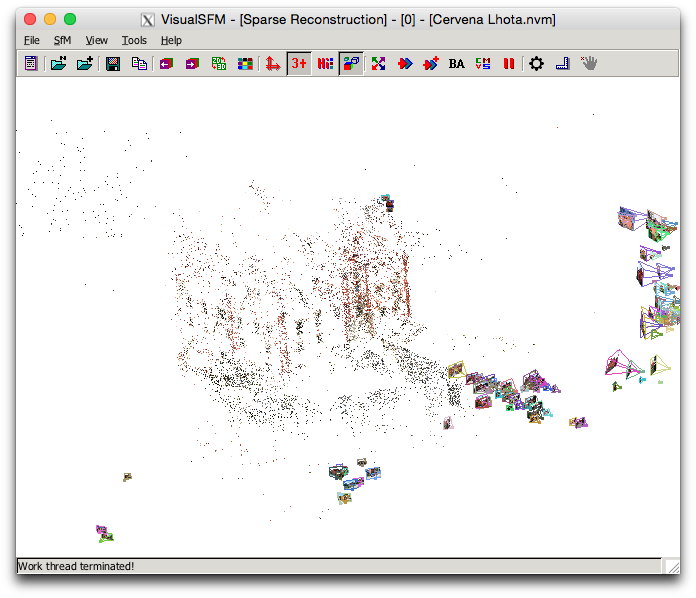
\includegraphics[keepaspectratio,width=14cm]{fig/VisualSFM.png}
	\end{center}
	\caption{The VisualSFM application GUI with sparse reconstruction of the Červená Lhota Castle.}
	\label{fig:visualsfm}
\end{figure}

\subsection*{Bundler}
Bundler is first well known Structure from Motion (SfM) system for unordered image collections from Noah Snavely. One of the first version of this Bundler system was used in the Photo Tourism project that was aqired by Microsoft and is now part of Photosynth. 

As other applications discussed, Bundler takes a set of images, image features, and image matches as input, and produces a 3D reconstruction of camera and sparse scene geometry as output. In order to get sparse point clouds, one has to run Bundler to get camera parameters, use the Bundle2PMVS program to convert the results into PMVS2 input and then run PMVS2. The system reconstructs the scene incrementally, a few images at a time, using a modified version of the Sparse Bundle Adjustment package of Lourakis and Argyros as the underlying optimization engine. Bundler has been successfully run on many Internet photo collections, as well as more structured collections. \cite{www:bundler}

\chapter{Methodology}
\label{chapter:methodology}
This chapter describes the process of 3D reconstruction from a set of images to the point cloud output. It puts the features detection, extraction and matching into context of 3D reconstruction. In order to select only inliers, the RUNSAC algorithmes filters the matched feature pairs. Then, using mathematical apparatus from chapter \ref{chapter:theoretical-background} the fundamental matrix and camera model are estimated. Finally, once we know the camera model, we can run dense reconstruction, creating the resulting point cloud.  
\section{3D Reconstruction Pipeline}
\subsection*{Feature Detection and Extraction}
\subsection*{Feature Matching}
\subsubsection*{RUNSAC}
\subsection*{Bundle Adjustment}
Camera Model and Fundamental Matrix Estimation
\subsection*{Dense Reconstruction}

\chapter{Results Evaluation}
\label{chapter:results_evaluation}

\chapter{Conclusion}
\label{chapter:conclusion}

%=========================================================================
